\newpage
\setcounter{figure}{0}

\section{Izgradnja 3D modela scene} % (fold)
\label{sec:Izgradnja 3D modela scene}

\subsection{Snimanje scene 3D kamerom i RGBDSlam programom} % (fold)
\label{sub:Snimanje scene 3D kamerom i RGBDSlam programom}
% RGBDSLAM allows to quickly acquire colored 3D models of objects and
% indoor scenes with a hand-held Kinect-style camera. 
Program RGBDSlam omogućava izgradnju 3D modela objekata i scena
u unutrašnjosti prostorija (oblak točaka u boji) rukom upravljanom 
kamerom tipa Kinect. Razvijen je suradnjom sveučilišta 
Albert-Ludwigs-Unversität\footnotemark[1] u Freiburgu i
Technische Universität München\footnotemark[2].
Slobodan je program objavljen pod GPLv3\footnotemark[3] licencom.
Izvorni kod je dostupan na Google code\footnotemark[4]
stranicama. U prilogu diplomskog rada nalaze se upute za prevođenje i
instaliranje programa. 

\footnotetext[1]{%
\href{http://www.informatik.uni-freiburg.de/~endres/}%
{Felix Endres} i \href{http://www.informatik.uni-freiburg.de/~hess/}%
{Juergen Hess} sa odijela \href{http://ais.informatik.uni-freiburg.de/}%
{Autonomous Intelligent Systems} koji vodi
\href{http://www.informatik.uni-freiburg.de/~burgard/}%
{Prof. Dr. Wolfram Burgard}.
}
\footnotetext[2]{%
\href{http://vision.in.tum.de/members/engelhan}%
{Nikolas Engelhard} sa odijela \href{http://vision.in.tum.de/}%
{Computer Vision Group} koji vodi
\href{http://vision.in.tum.de/members/sturmju}% 
{Dr. Juergen Sturm}.
}
\footnotetext[3]{%
GNU General Public License version 3 slobodna je licenca koja
osigurava osnovna prava slobodnih programa. Pravo na korištenje,
proučavanje, kopiranje i poboljšavanje. Izvor: 
\url{http://www.gnu.org/licenses/gpl-3.0.html}}

\footnotetext[4]{%
RGBDSlam program moguće je preuzeti sa \texttt{svn} programom sa stranice
\url{http://alufr-ros-pkg.googlecode.com/svn/trunk/rgbdslam\_freiburg/}%
}

\newpage
\subsubsection{Sažet opis rada RGBDSlam programa} % (fold)
\label{ssub:Sažet opis rada RGBDSlam programa}

\begin{figure}[h]
\renewcommand{\figurename}{Grafikon}
\centering
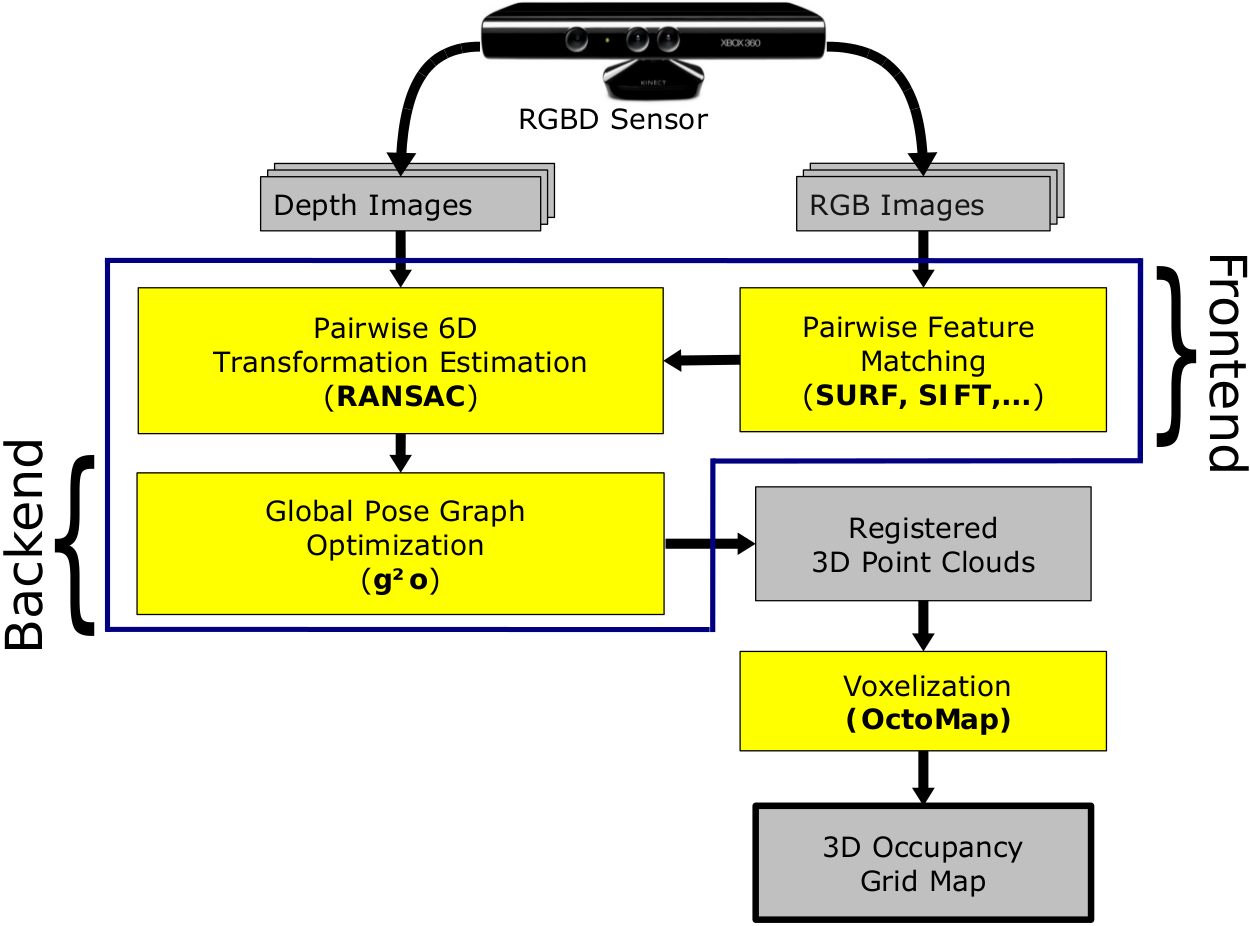
\includegraphics[scale=0.27]{figures/rgbdslam-overview.png}
\caption[]{Shematski pregled\footnotemark[1] RGBDSlam programa}
\label{fig:rgbdslam-overview}
\end{figure}

\footnotetext[1]{%
Shema je preuzeta iz znanstvenog rada ``An Evaluation of the RGB-D SLAM
System'' autora Endres, Hess, Burgard, Engelhard, Cremers,
Sturm~\cite{endres12icra}.
}

Kao što je vidljivo iz grafikona~\ref{fig:rgbdslam-overview} program je
podijeljen u četiri osnovna dijela. Prvi dio računa značajke iz ulaznih
slika u boji. RGBDSlam se oslanja na OpenCV~\cite{opencv_library}
biblioteku u kojoj su implementirani SURF~\cite{Bay06surf:speeded},
SIFT~\cite{Lowe04distinctiveimage} i ORB~\cite{1302} algoritmi za
pronalazak značajki. Zatim se te značajke sparuju sa značajkama iz
prethodnih slika. Drugi dio ispituje dubinu slika na lokacijama
izračunatih značajki. Usporedbom lokalnih deskriptora dobiva se
informacija o mogućim 3D korespondencijama točaka između bilo koje dvije
sličice.  Zatim je na temelju tih korespondencija estimirana relativna
transformacija između sličica upotrebom RANSACa. RANSAC Random Sample
Consensus~\cite{AICPub836:1981} je iterativna metoda estimiranja
parametara matematičkog modela iz promatranih mjerenja koja sadržavaju
šum i odudarajuće vrijednosti. RANSAC postupkom se uklanjaju netočne
korespodencije ostvarne na temelju lokalnih deskriptora. Kako parovi
estimiranih položaja između sličica nisu globalno konzistentni treći dio
programa optimizira graf položaja upotrebom g\textsuperscript{2}o
algoritma. {g\textsuperscript{2}o} General Framework for Graph
Optimization~\cite{kuemmerle11icra} je okvir otvorenog koda za
optimiziranje nelinearnih funkcija pogreške zasnovanih na grafu.
Algoritam u ovoj fazi daje globalno konzistentni 3D model promatrane
okoline predstavljen oblakom točaka u boji. Takav oblak točaka je
upotrebljen u diplomskom radu za stvaranje mreže trokuta.  RGBDSlam je
dizajniran da osim oblaka točaka generira i volumetrijski prikaz okoline
upotrebljavajući {OctoMap}~\cite{hornung13auro} biblioteku ali takav
prikaz nije korišten za potrebe ovog rada.

% subsubsection Sažet opis rada RGBDSlam programa (end)

\newpage
\subsubsection{Pokretanje RGBDSlam programa} % (fold)
\label{ssub:Pokretanje RGBDSlam programa}

Instaliran program pokreće se preko komandne linije koristeći
\texttt{roslaunch} koji je dio ROS~\cite{ros} biblioteke i alata
koji su detaljnije objašnjeni u poglavlju~\ref{sub:ROS biblioteka i
alati} Kao što je prikazano na slici~\ref{fig:running-rgbdslam}
\texttt{roslaunch} za parametar prima XML datoteku s ekstenzijom
\texttt{.launch} u kojoj su definirani parametri s kojima se pokreće
program.

\setcounter{figure}{0}
\begin{figure}[h]
\centering
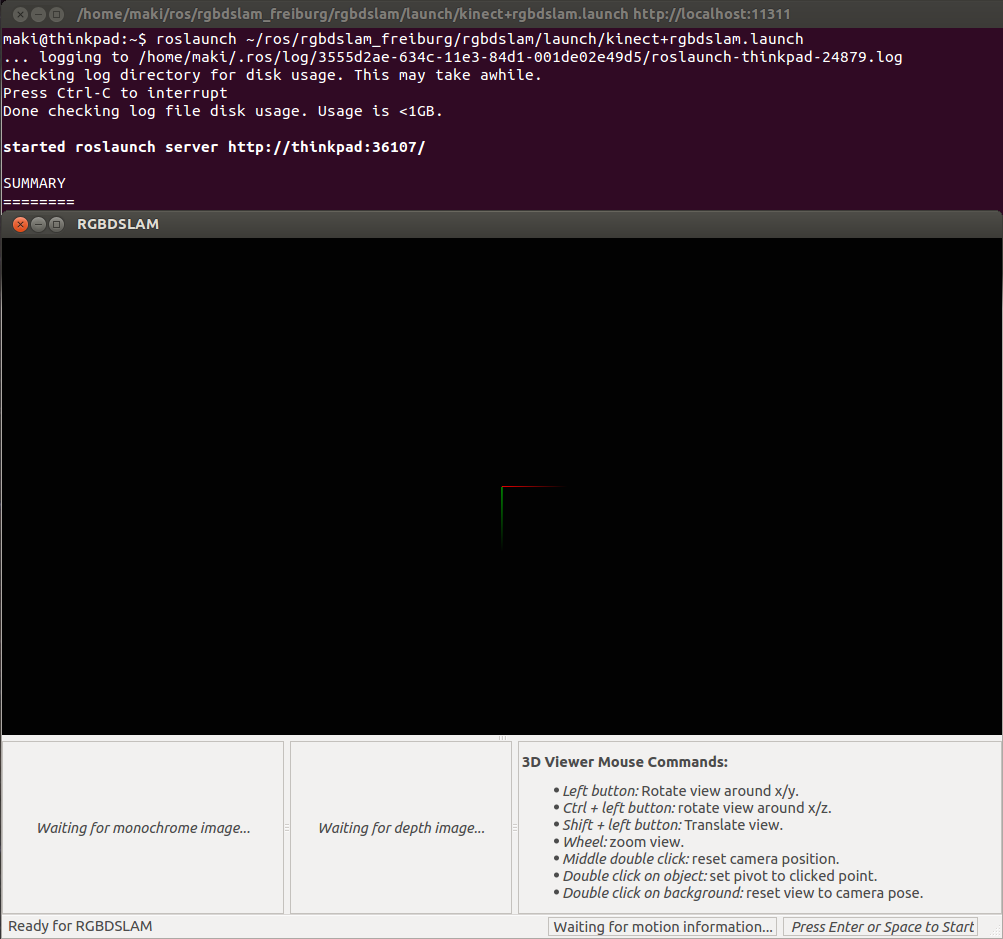
\includegraphics[scale=0.39]{figures/running-rgbdslam.png}
\caption{Prikaz pokretanja RGBDSlam programa iz komandne linije}
\label{fig:running-rgbdslam}
\end{figure}

Prilikom upotrebe RGBDSlama nije bilo potrebe za mijenjanjem zadanih
postavki te je korištena zadana \texttt{kinect+rgbdslam.launch}
datoteka za pokretanje. Program podržava dva načina rada, automatski i
ručni. Kod automatskog načina program neprestano uzima slike s kamere i
procesira ih, što u kratkom vremenu rezultira velikom količinom
podataka. Ručni način korisniku omogućava uzimanje slike na pritisak
tipke Enter.

% subsubsection Pokretanje RGBDSlam programa (end)

\newpage
\subsubsection{Snimanje scena RGBDSlam programom} % (fold)
\label{ssub:Snimanje scena RGBDSlam programom}

Za snimanje scena upotrijebljen je ručni način rada RGBDSlam programa.
Prednost ručnog načina rada je što snimatelj kontrolira broj slika
uzetih s kamere. Nedostatak je što je nezgodno jednoj osobi baratati s
kamerom, gledati u računalo i pritiskati Enter za slikanje. Zato je pri
snimanju scena sudjelovalo više osoba ili je korištena
skripta\footnotemark[1] koja umjesto korisnika šalje signal Enter
programu nakon proizvoljnog broja sekudni. Tijekom snimanja trebalo je
obratiti pozornost na značajke scene koja se snima kako bih program
mogao spariti značajke s prethodnom scenom. Tijekom izrade diplomskog
rada snimljeno je šest scena odnosno prostorija koje su obrađene u
poglavlju~\ref{sec:Rezultati} Snimljene scene su spremane u
\texttt{.pcd} formatu i kao takve korištene za daljnju obradu u
diplomskom radu.

\footnotetext[1]{%
Skripta za slikanje dostupna je na DVDu i na web stranici
\url{http://github.com/msvalina/pcl-surface-mesh-reconstruction}}

% subsubsection Snimanje scena RGBDSlam programom (end)

% subsection Snimanje scene 3D kamerom i RGBDSlam programom (end)

\newpage
\subsection{Izgradnja 3D modela scene pomoću mreže trokuta} % (fold)
\label{sub:Izgradnja 3D modela scene pomoću mreže trokuta}

Izgradnja 3D modela scene pomoću mreže trokuta je implementirana u
programu nazvanom \texttt{mesh-reconstruction}.\footnotemark[1]
Program se intenzivno oslanja na biblioteku PointCloud koja je opisana u
podpoglavlju \ref{sub:Biblioteka Pointcloud} Kao što je vidljivo iz
grafikona \ref{fig:flowchart} program je podijeljen u pet osnovnih
funkcija:
\begin{itemize}
    \item Učitavanje oblaka točaka snimljenih RGBDSlam programom.
    \item Reduciranje oblaka točaka.
    \item Uklanjanje pogrešaka pri mjerenju.
    \item Stvaranje i zapisivanje mreže trokuta.
    \item Prikaz mreže trokuta.
\end{itemize}

\footnotetext[1]{%
Program \texttt{mesh-reconstruction} slobodan je program dostupan pod
uvijetima MIT licence. Izvorni kod se nalazi na DVDu i na web stranici
\href{http://github.com/msvalina/}%
{\texttt{github.com/msvalina/}}}

\setcounter{figure}{1}
\begin{figure}[h]
\renewcommand{\figurename}{Grafikon}
\centering
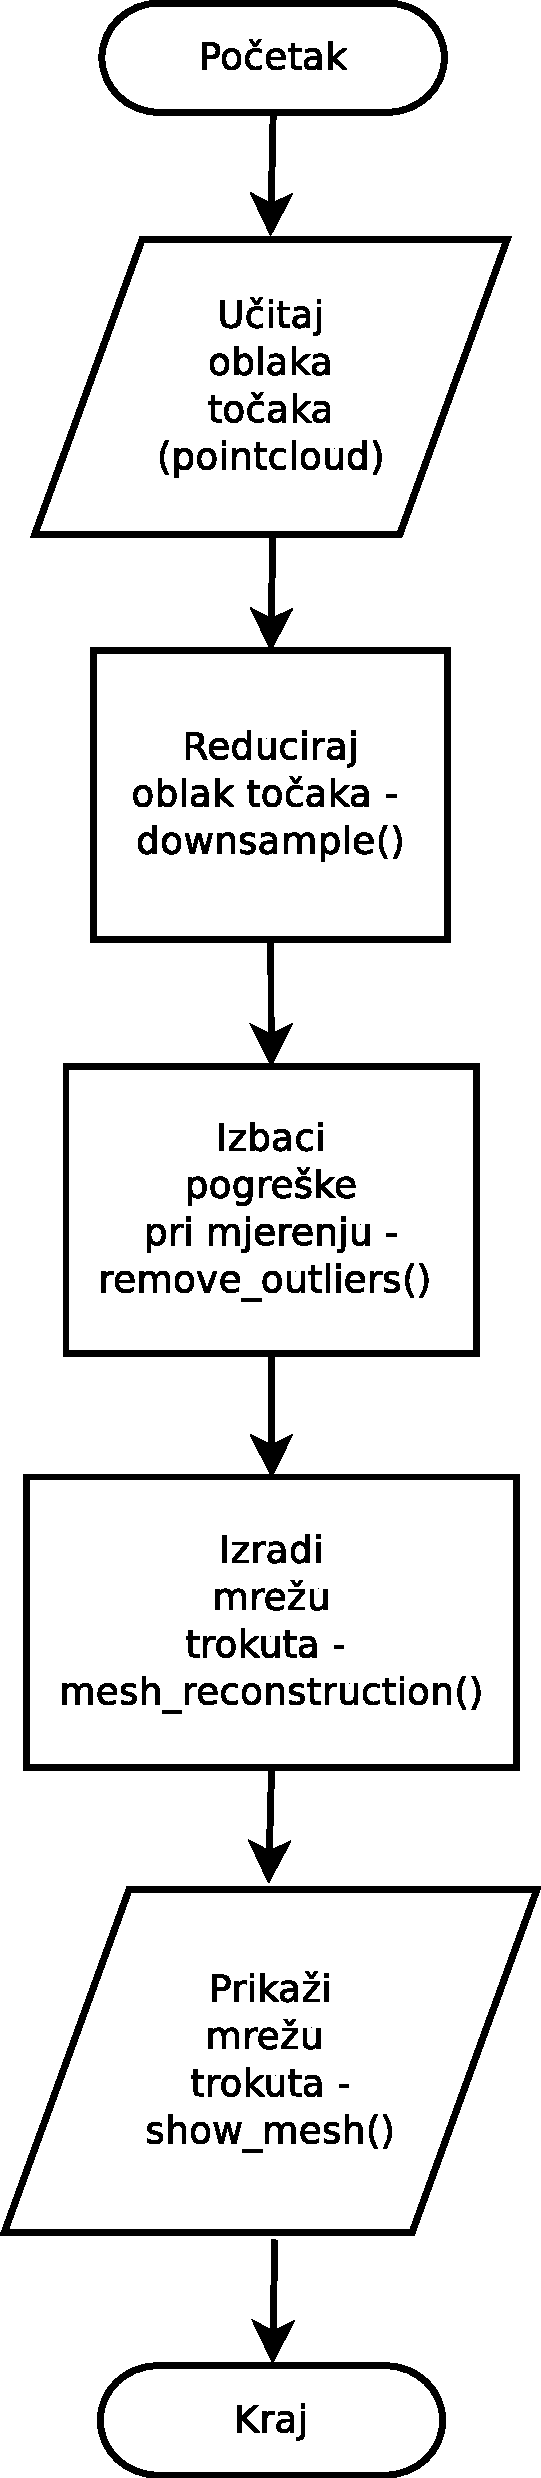
\includegraphics[scale=0.5]{figures/flowchart.pdf}
\caption{Dijagram toka programa \texttt{mesh-reconstruction} }
\label{fig:flowchart}
\end{figure}

U sljedećim podpoglavljima dan je pregled funkcija i PCL~\cite{pcl}
klasa na kojima se baziraju. Također na
slici~\ref{fig:running-mesh-reconstruction} se vidi kako izgleda
pokretanje programa, što sve ispisuje na standardni izlaz te kako
prikazuje mrežu trokuta.

\newpage
% Reset counter becouse Grafikon and figures should have diff counters
\setcounter{figure}{1}
\begin{figure}[h]
\centering
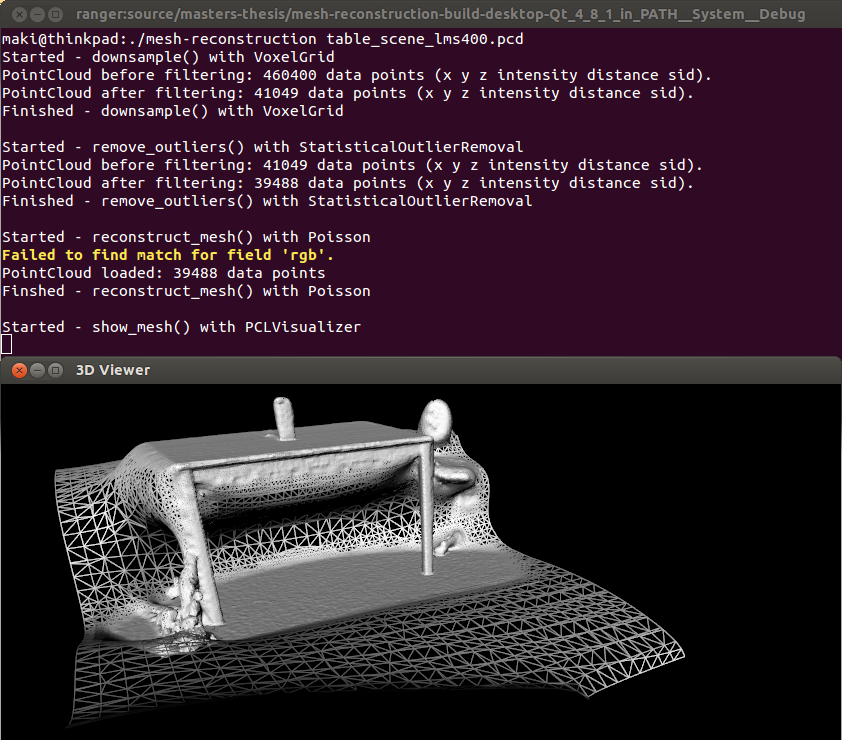
\includegraphics[scale=0.5]{figures/running-mesh-reconstruction.png}
\caption{Prikaz pokretanja programa \texttt{mesh-reconstruction} iz
terminala}
\label{fig:running-mesh-reconstruction}
\end{figure}

\newpage
\subsubsection{Pregled \texttt{main()} funkcije} % (fold)
\label{ssub:Pregled main funkcije}
\begin{lstlisting}[label=lstMain,caption={Izvorni kod
\texttt{main()} funkcije }]
int main (int argc, char *argv[])
{
    downsample (argc, argv);
    remove_outliers (argc, argv);
    pcl::PolygonMesh mesh_of_triangles;
    reconstruct_mesh (argc, argv, mesh_of_triangles);
    show_mesh (mesh_of_triangles);
    return 0;
}
\end{lstlisting}
Kao što se vidi iz ispisa koda~\ref{lstMain} ideja je da funkcija bude
što manja te da se iz nje samo pozivaju druge funkcije. 

% subsubsection Pregled tt (end)

\subsubsection{Učitavanje oblaka točaka} % (fold)
\label{ssub:Učitavanje oblaka točaka}
Program se sastoji od funkcija \texttt{downsample},
\texttt{remove\_outliers}, \texttt{reconstruct\_mesh} i
\texttt{show\_mesh}. Na početku svake funkcije program učitava oblak
točaka, obrađuje ga i zapisuje na izlazu iz funkcije kako bi prije i
poslije svake operacije bio dostupan. Za to koristi \texttt{PCDReader} i
\texttt{PCDWriter} klase. Predložak takvog koda se nalazi u ispisu
koda~\ref{lstUcitavanjeOblaka} Nakon učitavanja oblaka točaka
\texttt{reader} objektom, nad njim se vrše operacije npr.  reduciranje
oblaka točaka. Nakon toga kreiranjem i korištenjem \texttt{writer}
objekta promjenji oblak se zapisuje u datoteku.

\begin{lstlisting}[label=lstUcitavanjeOblaka, caption={Predložak izvornog
koda za učitavanje oblaka točaka}]
    // Init cloud variables 
    pcl::PCLPointCloud2::Ptr cloud (new pcl::PCLPointCloud2());
    pcl::PCLPointCloud2::Ptr cloud_filtered (new pcl::PCLPointCloud2());

    // Fill in the cloud data
    pcl::PCDReader reader;
    reader.read ("pointcloud.pcd", *cloud);
    /* 
     * Do something with cloud e.g. downsample pointcloud
     */
    // Write cloud to a file
    pcl::PCDWriter writer;
    writer.write ("pointcloud-downsampled.pcd",
            *cloud_filtered, Eigen::Vector4f::Zero(),
            Eigen::Quaternionf::Identity(), false);
\end{lstlisting}

% subsubsection Učitavanje oblaka točaka (end)

\newpage
\subsubsection{Reduciranje oblaka točaka} % (fold)
\label{ssub:Reduciranje oblaka točaka}
Reduciranje obalaka točaka ne unosi bitne gubitake informacije, a izvodi se
zbog lakše daljnje obrade oblaka. Izvodi se pomoću \texttt{VoxelGrid}
klase i implementirano je u \texttt{downsample()} funkciji. Dijelovi
funkcije prikazani su u ispisu koda~\ref{lstReduciranje}
\texttt{VoxelGrid} dolazi od riječi \textit{volume pixel grid} i
predstavlja niz malih kocaka u prostoru.

\begin{lstlisting}[label=lstReduciranje, caption={Dio izvornog koda za
reduciranje točaka iz funkcije \texttt{downsample()} }]
    // Create the filtering object
    pcl::VoxelGrid<pcl::PCLPointCloud2> vg;
    vg.setInputCloud (cloud);
    // voxel size to be 1cm^3
    vg.setLeafSize (0.01f, 0.01f, 0.01f);
    vg.filter (*cloud_filtered);
\end{lstlisting}

Kao što se vidi iz ispisa koda~\ref{lstReduciranje} nakon kreiranja
objekta \texttt{vg} predaje mu se oblak točaka nad kojim se vrši
reduciranje. Postavlja se veličina kocke (\textit{voxel}) u našem
slučaju to je 1cm\textsuperscript{3}. Nad tim oblakom prilikom
filtriranja će se kreirati mreža kocaka te će se sve točke unutar jedne
kocke zamjeniti centralnom točkom. Tim postupkom značajno se smanjuje
broj točaka u oblaku kao što je vidljivo iz
slike~\ref{fig:tablescene-downsample}

\begin{figure}[h]
\centering
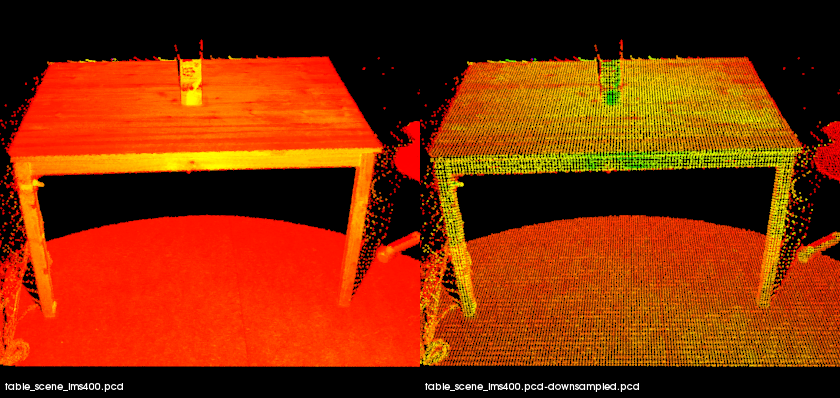
\includegraphics[scale=0.5]{figures/tablescene-downsampling-example.png}
% If there is \footnote in caption brackets [] must be used in \caption
\caption[description for List of Figures]{%
    Oblak točaka \textit{table\_scene}\footnotemark[1] lijevo prije
    \texttt{downsample()} 460400 točaka i poslije desno 41049 točaka}
\label{fig:tablescene-downsample}
\end{figure}

\footnotetext[1]{Oblak točaka \texttt{table\_scene\_lms400.pcd} je
objavljen pod uvijetima BSD licence izvor: 
\href{https://github.com/PointCloudLibrary/data/blob/master/tutorials%
/table\_scene\_lms400.pcd}{\texttt{ %
github.com/PointCloudLibrary/\dots/table\_scene\_lms400.pcd}}}

% subsubsection Reduciranje oblaka točaka (end)

\newpage
\subsubsection{Uklanjanje pogrešaka pri mjerenju} % (fold)
\label{ssub:Uklanjanje pogrešaka pri mjerenju}
Pogreške pri mjerenju su sastavni dio svakog mjernog uređaja. U slučaju
Kinect senzora često se javljaju odudarajuće vrijednosti (engl.
\textit{outliers}). PointCloud biblioteka ima ugrađenu
\texttt{StatisticalOutlierRemoval} klasu koja uklanja odudarajuće
vrijednosti, a implementirana je u funkciji
\texttt{remove\_outlieres()}. Iz ispisa koda~\ref{lstUklanjanje} se
vidi kako se klasa koristi.

% minipage ensures that listing won't be split between pages
% but it seams like it's pushing whole box slightly to the right
% \begin{minipage}{\textwidth}
\begin{lstlisting}[label=lstUklanjanje, caption={Dio izvornog koda za 
    uklanjanje odudarajaućih vrijednosti iz funkcije \texttt{remove\_outliers()} }]
    // Create the filtering object
    pcl::StatisticalOutlierRemoval<pcl::PCLPointCloud2> sor;
    sor.setInputCloud (cloud);
    // Set number of neighbors to analyze
    sor.setMeanK (50);
    sor.setStddevMulThresh (1.0);
    sor.filter (*cloud_filtered);
\end{lstlisting}
% \end{minipage}

Nakon kreiranja objekta \texttt{sor} i predavanja oblaka postavljena su
još dva parametra. Prvi \texttt{setMeanK} je broj susjednih točaka koje
će filter analizirati. Drugi \texttt{setStddevMulThresh} postavlja
multiplikator praga standardne devijacije. Algoritam dva puta prolazi
kroz oblak točaka. U prvoj iteraciji računa srednju vrijednost
udaljenosti svake točke do njenih K susjeda. Zatim računa očekivanje
\(\mu\) i standardnu devijaciju \(\sigma\) svih udaljenosti kako bi
mogao odrediti prag udaljenosti. Prag udaljenosti je određen jednadžbom
\(\mu+\texttt{StddevMulThresh}\cdot\sigma\). U sljedećoj iteraciji točke
će biti označene kao outlier ukoliko su njihove srednje vrijednosti
udaljenosti od susjeda veće od praga. Rezultati rada funkcije se vide na
slici~\ref{fig:tablescene-outliers}
 
\begin{figure}[h]
\centering
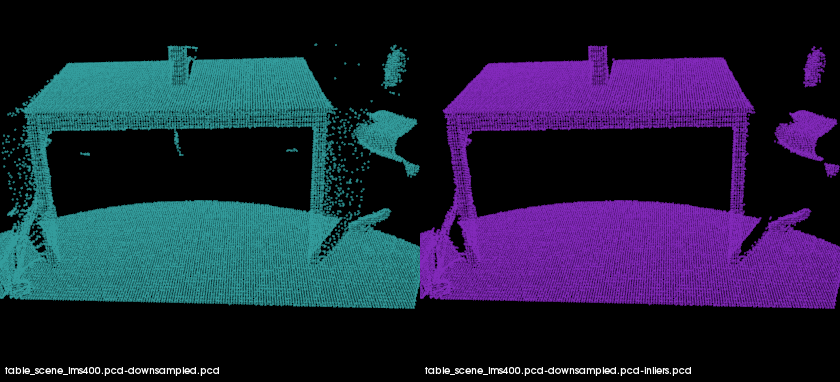
\includegraphics[scale=0.5]{figures/tablescene-remove-outliers-example.png}
\caption{Oblak točaka lijevo poslije \texttt{downsample()} 41049 točka i desno poslije
\texttt{remove\_outliers()} 39488 točka }
\label{fig:tablescene-outliers}
\end{figure}

% subsubsection Uklanjanje pogrešaka pri mjerenju (end)

\newpage
\subsubsection{Stvaranje i zapisivanje mreže trokuta} % (fold)
\label{ssub:Stvaranje i zapisivanje mreže trokuta}

Nakon pripreme oblaka točaka funkcijama \texttt{downsample()} i
\texttt{remove\_outliers()} slijedi stvaranje mreže trokuta unutar
funkcije \texttt{mesh\_reconstruction()}. Stvaranje mreže trokuta se
može podijeliti u tri koraka. Prvi je estimiranje normala nad oblakom
točaka. Drugi je spajanje estimiranih normala i oblaka točaka u
zajedniči oblak točaka s normalama. Treći korak je pozivanje algoritma
za stvaranje mreže nad novo stvorenim oblakom.

\begin{lstlisting}[label=lstStvaranje1, caption={Dio izvornog koda za
    estimaciji normala iz funkcije \texttt{reconstruct\_mesh()} }]
    // Normal estimation
    pcl::NormalEstimation<PointType, Normal> normEst;
    pcl::PointCloud<Normal>::Ptr normals (new pcl::PointCloud<Normal>);
    
    // Create kdtree representation of cloud, 
    // and pass it to the normal estimation object. 
    pcl::search::KdTree<PointType>::Ptr tree (new
            pcl::search::KdTree<PointType>);
    tree->setInputCloud (cloud);
    normEst.setInputCloud (cloud);
    normEst.setSearchMethod (tree);
    // Use 20 neighbor points for estimating normal
    normEst.setKSearch (20);
    normEst.compute (*normals);
\end{lstlisting}

Iz ispisa koda~\ref{lstStvaranje1} se vidi da je prije estimiranja
normala nad oblakom točaka potrebno inicijalizirati objekt za
spremanje normala i za estimaciju. Nakon toga definira se
stablo za pretraživanje oblaka tipa \texttt{KdTree}.\footnotemark[1]
Stablu se tada predaje oblak za pretraživanje. Objektu za
estimaciju \texttt{normEst} tada se predaje oblak i stablo te broj
susjednih točaka nad kojima se vrši estimacija
normala\footnotemark[2]. 

\footnotetext[1]{%
K dimenzionalno stablo~\cite{Moore1991} je detaljno objašnjeno i na
stranici \url{http://%
pointclouds.org/documentation/tutorials/kdtree\_search.php}%
}
\footnotetext[2]{%
Estimacija normala detaljno je objašnjena na stranici \url{http://%
pointclouds.org/documentation/tutorials/normal\_estimation.php}%
}

Nakon estimacije normala slijedi spajanje estimiranih normala i oblaka u
novi oblak točaka s normalama. Kao što je prikazano u ispisu
koda~\ref{lstStvaranje2} Taj oblak točaka je prikazan na 
slici~\ref{fig:tablescene-normals}

\newpage
\begin{lstlisting}[label=lstStvaranje2,caption={Dio izvornog koda za
    stvaranju mreže iz funkcije \texttt{reconstruct\_mesh()} }]
    // Concatenate the XYZ and normal fields
    pcl::PointCloud<PointTypeN>::Ptr cloud_with_normals (new
            pcl::PointCloud<PointTypeN>);
    pcl::concatenateFields (*cloud, *normals, *cloud_with_normals);
    // cloud_with_normals = cloud + normals

    // Create search tree 
    pcl::search::KdTree<PointTypeN>::Ptr tree2 (new
            pcl::search::KdTree<PointTypeN>);
    tree2->setInputCloud (cloud_with_normals);

    // Initialize objects 
    // psn - for surface reconstruction algorithm
    // triangles - for storage of reconstructed triangles
    pcl::Poisson<PointTypeN> psn;
    pcl::PolygonMesh triangles;

    psn.setInputCloud(cloud_with_normals);
    psn.setSearchMethod(tree2);
    psn.reconstruct (triangles);
    psn.setOutputPolygons(false);
\end{lstlisting}

Nad stvorenim oblakom s normalama stvara se stablo za pretraživanje.
Zatim se inicijaliziraju objekti \texttt{psn} i \texttt{triangles}.
\texttt{psn} predstavlja \texttt{Poisson}\footnotemark[1] algoritam za
stvaranje mreže trokuta. \texttt{triangles} je objekt tipa
\texttt{PolygonMesh} za spremanje izračunatih koordinata trokuta.
Algoritmu se sada predaje ulazni oblak, stablo pretraživanja i poziva se
rekonstrukcija.

\footnotetext[1]{%
Poisson algoritam su razvili Michael Kazhdan i Matthew Bolitho,
objavljen je pod BSD licencom. Izvor: \url{http://www.cs.jhu.edu/~misha/Code/%
PoissonRecon/Version5.5/}}

\begin{figure}[h]
\centering
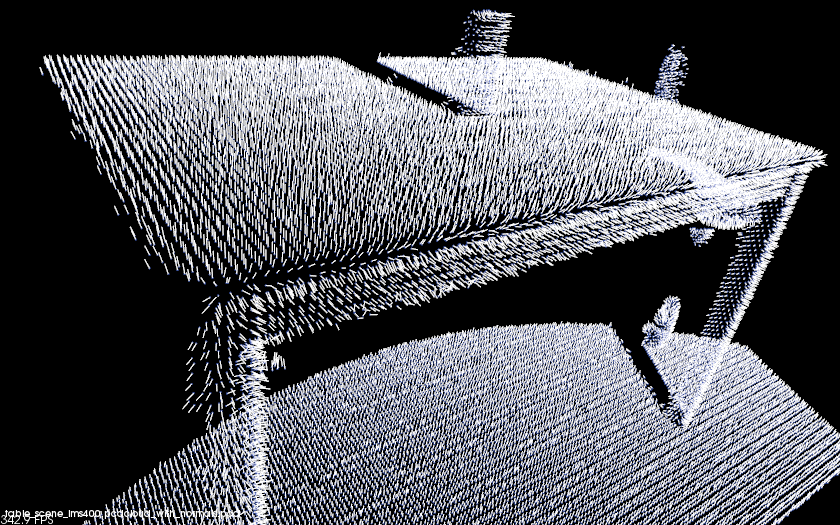
\includegraphics[scale=0.4]{figures/tablescene-normals.png}
\caption{Prikaz oblaka točaka \texttt{tablescene} s estimiranim
normalama }
\label{fig:tablescene-normals}
\end{figure}

Ispis koda~\ref{lstStvaranje3} prikazuje korištenje klase
\texttt{saveVTKFile} za spremanje objekta \texttt{triangles} u datoteku
s vtk ekstenzijom.

\begin{lstlisting}[label=lstStvaranje3,caption={Dio izvornog koda za
    zapisivanju mreže iz funkcije \texttt{reconstruct\_mesh()} }]
    // Write reconstructed mesh
    if (argc < 2){
        pcl::io::saveVTKFile
            ("pointcloud-downsampled-outliers-mesh.vtk",
             triangles);
    }
    else {
        std::string str;
        str.append(argv[1]).append("-mesh.vtk");
        pcl::io::saveVTKFile (str, triangles);
    }
\end{lstlisting}

% subsubsection Stvaranje i zapisivanje mreže trokuta (end)

\newpage
\subsubsection{Prikazivanje mreže trokuta} % (fold)
\label{ssub:Prikazivanje mreže trokuta}
Prikazivanje mreže trokuta omogućava \texttt{PCLVisualizer} klasa. Ista
klasa se koristi u komandno linijskom programu za prikaza oblaka točaka
\texttt{pcl\_vieweru}. U ispisu koda~\ref{lstPrikaz} se vidi
jednostavnost upotrebe klase. Nakon kreiranja objekta \texttt{viewer} i
postavljanja parametara poziva se beskonačna petlja. Metoda
\texttt{spinOnce()} izvodi crtanje mreže, prikazivanje na ekranu i
daje \texttt{vieweru} vremena za procesiranje i time omogućava
interaktivnost s mrežom. Klikom na tipku \texttt{q} izlazi se iz petlje
i program završava. Slika~\ref{fig:tablesecne-mesh-perspectives}
prikazuje izgled mreže iz četiri pogleda.

\begin{figure}[H]
\centering
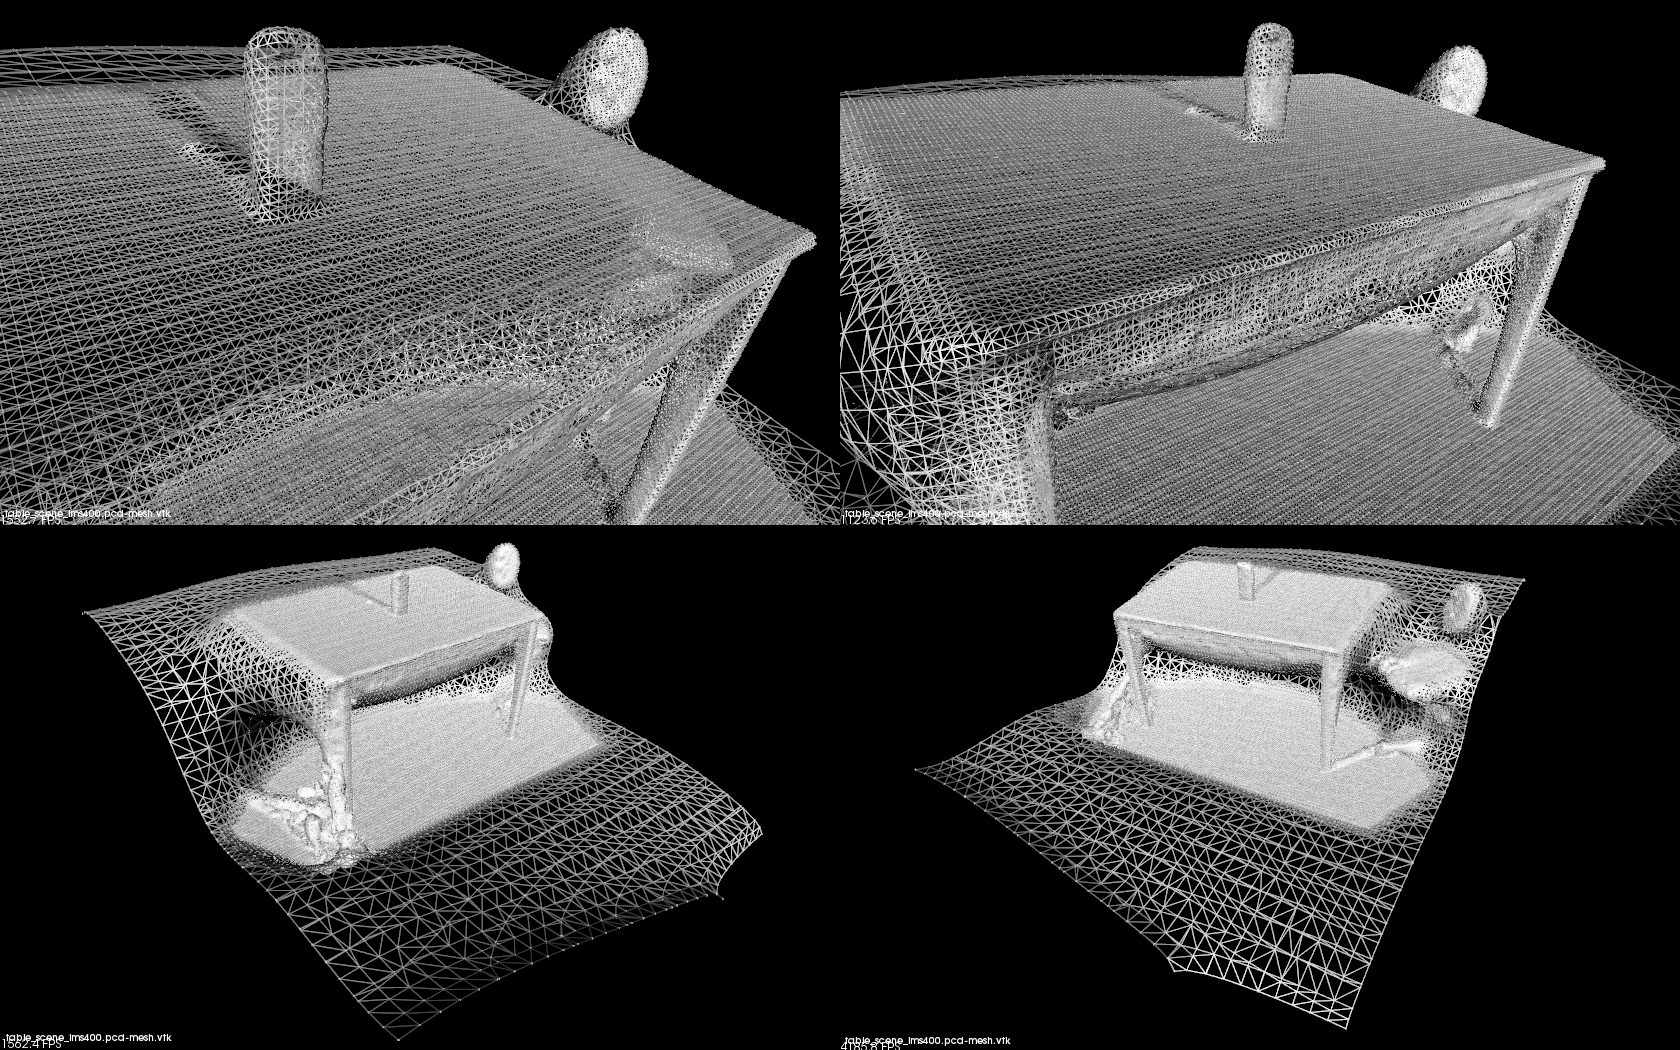
\includegraphics[scale=0.24]{figures/tablescene-mesh-perspectives.png}
\caption{Prikaz mreže trokuta funkcijom \texttt{show\_mesh()} }
\label{fig:tablesecne-mesh-perspectives}
\end{figure}

\begin{lstlisting}[label=lstPrikaz,caption={Izvorni kod funkcije
\texttt{show\_mesh()} }]
void show_mesh (const pcl::PolygonMesh& mesh_of_triangles)
{
    std::cout << "Started - show_mesh() with PCLVisualizer\n";
    // Create viewer object and show mesh
    boost::shared_ptr<pcl::visualization::PCLVisualizer> viewer (new
          pcl::visualization::PCLVisualizer ("3D Viewer"));
    viewer->setBackgroundColor (0, 0, 0);
    viewer->addPolygonMesh (mesh_of_triangles, "sample mesh");
    viewer->initCameraParameters (); 
    while (!viewer->wasStopped ())
    {
        viewer->spinOnce (100); 
        boost::this_thread::sleep 
            (boost::posix_time::microseconds (100000));
    }
    std::cout << "Finshed - show_mesh() with PCLVisualizer\n";
}
\end{lstlisting}


% subsubsection Prikazivanje mreže trokuta (end)

% subsection Izgradnja 3D modela scene pomoću mreže trokuta (end)

\newpage
\subsubsection{Grafičko sučelje programa} % (fold)
\label{ssub:Grafičko sučelje programa}

Osim komandno linijske verzije programa izrađena je i verzija s
grafičkim sučeljem. Grafičko sučelje je napravljeno upotrebom Qt okvira.
Qt je C++ višeplatformski okvir za razvijanje aplikacija i korisničkih
sučelja. Na slici~\ref{fig:mesh-gui} se vidi izgled programa.

\begin{figure}[h]
\centering
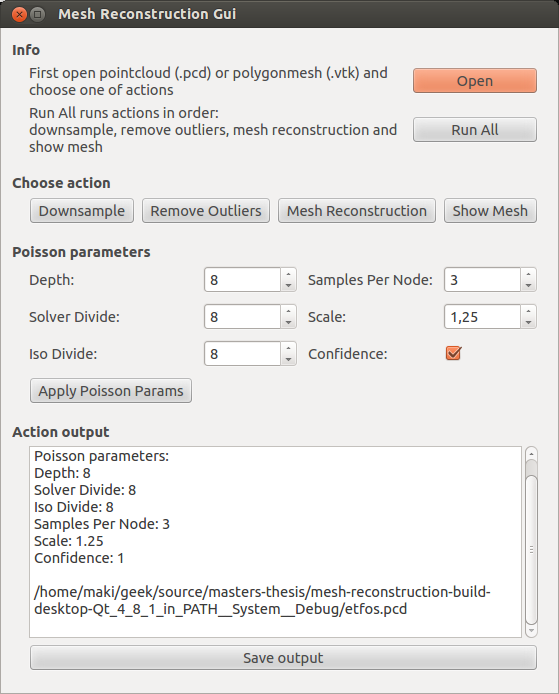
\includegraphics[scale=0.5]{figures/mesh-reconstruction-gui.png}
\caption{Prikaz glavnog prozora programa \texttt{mesh-reconstruction} }
\label{fig:mesh-gui}
\end{figure}

Sučelje programa je jednostavno i jasno te se sastoji od četiri sekcije
i dva prozora. Glavni prozor \texttt{Mesh Reconstruction Gui} prikazan
je na slici~\ref{fig:mesh-gui}, a prozor za prikazivanje mreže trokuta
\texttt{Visualisation} prikazan je na slici~\ref{fig:gui-2.png}. \\

\textbf{Prozor \texttt{Mesh Reconstruction Gui}} 
\begin{itemize}
    \item \textbf{Info} sekcija sadrži kratak opis i dugmad:
        \begin{itemize}
            \item \texttt{Open} za odabir datoteke s oblakom točaka
                (\texttt{.pcd}) odnosno datoteke s mrežom trokuta
                (\texttt{.vtk}).
            \item \texttt{Run All} za pokretanje svih akcija nad
                odabranim oblakom točaka.
        \end{itemize}
    \item \textbf{Choose action} sekcija sadrži dugmad:
        \begin{itemize}
            \item \texttt{Downsample} za reduciranje oblaka točaka.
            \item \texttt{Remove Outliers} za izbacivanje odudarajućih
                vrijednosti.
            \item \texttt{Mesh Reconstruction} za izgradnju mreže
                trokuta.
            \item \texttt{Show Mesh} za prikaz izrađene mreže trokuta.
        \end{itemize}
    \item \textbf{Poisson parameters} sekcija prikazuje parametre 
        Poisson algoritma za rekonstrukciju površine. Parametri i
        njihove vrijednosti su opisani u
        podpoglavlju~\ref{ssub:Parametri Poisson algoritma}
    \item \textbf{Action output} sekcija prikazuje ispis informacija
        pojedinih akcija te ima dugme \texttt{Save Output} za spremanje
        tektsa.
\end{itemize}
\textbf{Prozor Visualisation} 
\begin{itemize}
    \item Vizualizira kreiranu mrežu trokuta. Sadrži dva dugma:
        \begin{itemize}
            \item \texttt{Surfce representation} prikazuje mrežu trokuta
                pomoću površine.
            \item \texttt{Wireframe representation} prikazuje mrežu
                trokuta upotrebom trokutića.
        \end{itemize}
\end{itemize}

\begin{figure}[h]
\centering
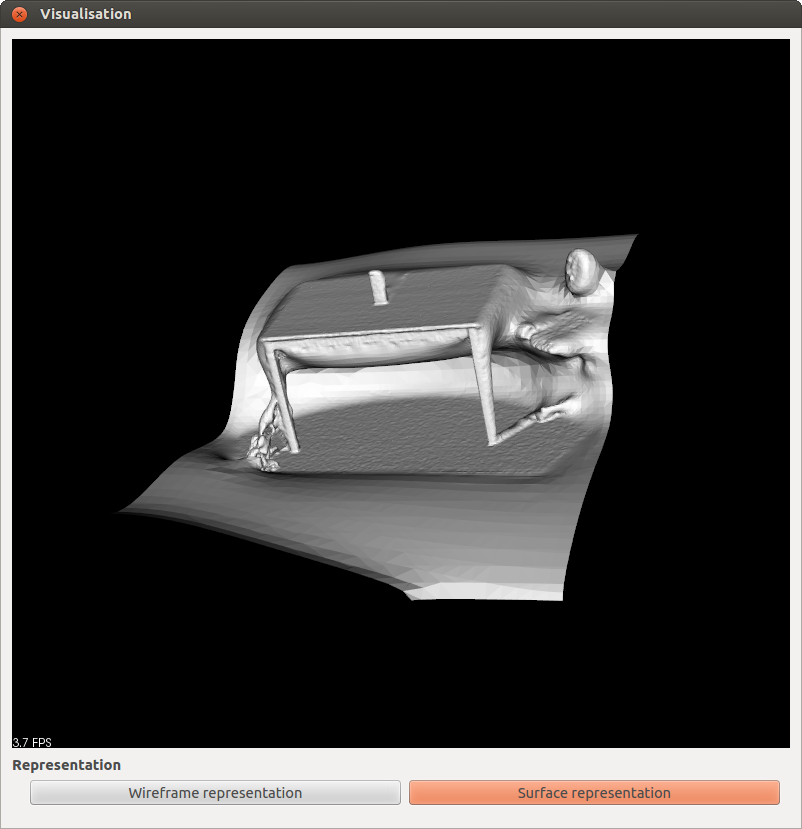
\includegraphics[scale=0.4]{figures/gui-2.png}
\caption{Prikaz prozora za vizualizaciju mreže trokuta}
\label{fig:gui-2.png}
\end{figure}

% subsubsection Grafičko sučelje programa (end)

% section Izgradnja 3D modela scene (end)
